% Very simple template for lab reports. Most common packages are already included.
\documentclass[a4paper, 11pt]{article}
\usepackage[utf8]{inputenc} % Change according your file encoding
\usepackage{graphicx}
\usepackage{url}
\usepackage{listings}
\usepackage[listings]{tcolorbox}
\usepackage{xcolor}
\usepackage{xcolor}
\usepackage{float} 
\usepackage{placeins} 

% Define a custom boxed listing environment
\newtcblisting{mylisting}{
  colback=gray!5!white, colframe=black!75!white,
  listing only,
  left=2mm, right=2mm, top=1mm, bottom=1mm,
  boxrule=0.5pt, arc=2mm
}

%opening
\title{Report 2: Routy, a small Routing Protocol}
\author{Lorenzo Deflorian}
\date{\today{}}

\begin{document}

\maketitle

\section{Introduction}

The main goal of this assignment was to implement a link-state routing protocol using the Dijkstra algorithm. The protocol should be able to handle dynamic changes in the network topology, such as link failures and recoveries, and update the routing tables accordingly. 

\section{Main problems and solutions}

The main challenge was to implement the Dijkstra algorithm correctly, ensuring that the routing tables are updated to reflect the current state of the network. Once the algorithm was implemented, I tested it on a small network topology, consisting of 5 routers, divided into two areas, running on two different Erlang nodes.

\subsection{Network Topology}

We start by defining the network topology as shown in Figure \ref{fig:network_topology}. We divide the whole network into two areas, running on two different Erlang nodes. We call the first area "Italy", which contains routers r1 (Rome), r2 (Milan), r3 (Turin), while the second area, "Spain", contains routers r4 (Barcelona), r5 (Madrid).

\begin{figure}[H]
  \centering
  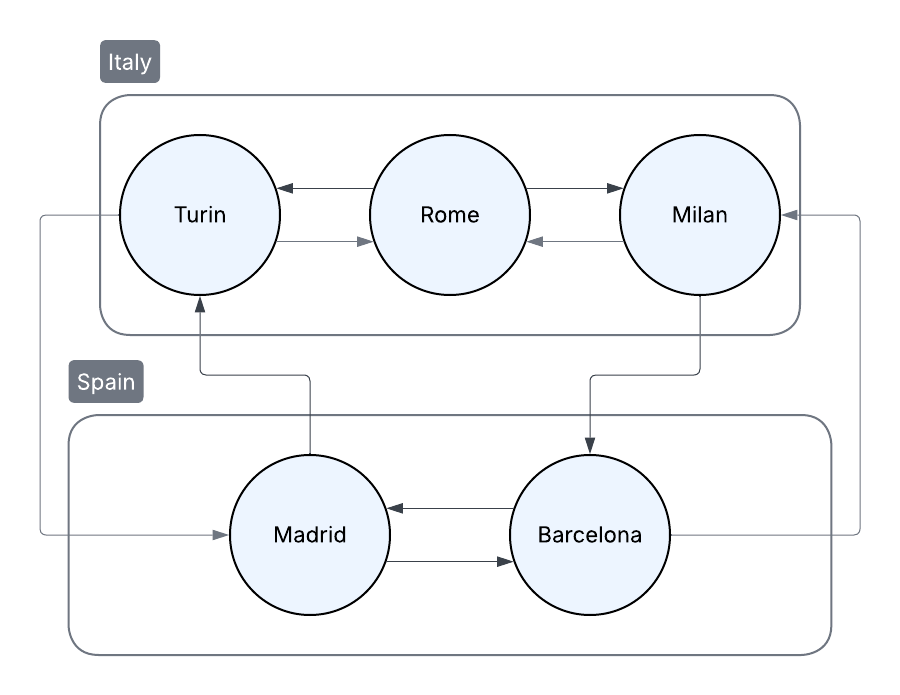
\includegraphics[width=0.9\linewidth]{network_topology.png}
  \caption{Network Topology}
  \label{fig:network_topology}
\end{figure}
\FloatBarrier

The connections between the routers are also shown in Figure \ref{fig:network_topology}. We set bidirectional links, all with the same cost.

\section{Evaluation}

\subsection{Testing the implementation}
After setting up the network topology as described above, we call the \texttt{broadcast} and \texttt{update} functions on each router to propagate the link-state information and compute the initial routing tables. 

\subsubsection{Initial message routing}

Let's send a message from Rome (r1) to Madrid (r5) and see how it is routed through the network.

\begin{mylisting}
(italy@DORORO)1> r1 ! {send, madrid, "Hello there"}.
rome: routing message "Hello there"
rome: gateway resolved to turin
{send,madrid,"Hello there"}
turin: routing message "Hello there"
turin: gateway resolved to madrid
\end{mylisting}



\begin{mylisting}
(spain@DORORO)1> madrid: routing message "Hello there"
madrid: received message "Hello there"
\end{mylisting}

As we can see, the message is correctly routed through the shortest path, which is \textbf{Rome} $\to$ \textbf{Turin} $\to$ \textbf{Madrid}.

\subsubsection{Simulating a link failure}

Let's simulate a link failure between Turin (r3) and Madrid (r5) by removing the connection between them. We also need to update the routing tables in both areas and propagate the changes through the network.


\begin{mylisting}
(italy@DORORO)2> r1 ! {remove, turin}.
{remove,turin}
(italy@DORORO)3> test:update_italy().
ok
\end{mylisting}


\begin{mylisting}
(spain@DORORO)2> test:update_spain().
ok
\end{mylisting}

Now, let's send the same message from Rome (r1) to Madrid (r5) again:

\begin{mylisting}
(italy@DORORO)4> r1 ! {send, madrid, "Hello there"}.
rome: routing message "Hello there"
rome: gateway resolved to milan
{send,madrid,"Hello there"}
milan: routing message "Hello there"
milan: gateway resolved to barcelona
\end{mylisting}

\begin{mylisting}
(spain@DORORO)3> barcelona: routing message "Hello there"
barcelona: gateway resolved to madrid
madrid: routing message "Hello there"
madrid: received message "Hello there"
\end{mylisting}

As we can see, the message is still correctly routed through the network, but this time the path is \textbf{Rome} $\to$ \textbf{Milan} $\to$ \textbf{Barcelona} $\to$ \textbf{Madrid}, which is the new shortest path after the link failure.

\section{Conclusions}

In this report, we have described the implementation and testing of a link-state routing protocol using the Dijkstra algorithm. We have shown how the protocol can handle dynamic changes in the network topology, such as link failures and recoveries, and update the routing tables accordingly. The testing results demonstrate that the protocol is able to find the shortest path between any two routers in the network, even in the presence of link failures.


To further improve the protocol, we could consider implementing link cost variations, where different links have different costs, and the Dijkstra algorithm would need to take these costs into account when computing the shortest path. 

Another possible improvement would be to implement an automatic mechanism for routers to detect link failures and changes in the network topology, rather than relying on manual updates.

This could be achieved by implementing a heartbeat mechanism, in which routers periodically send "hello" messages to their neighbors to check if they are still reachable. If a router does not receive a "hello" message from a neighbor within a certain time frame, it can assume that the link to that neighbor has failed and update its routing table accordingly.

\section{The world}

Let's try to see if we can route a message from our machine to another node running on a different machine. To do this i have asked the help of a friend, Riccardo Fragale, who has set up his topology as follows:

\begin{center}
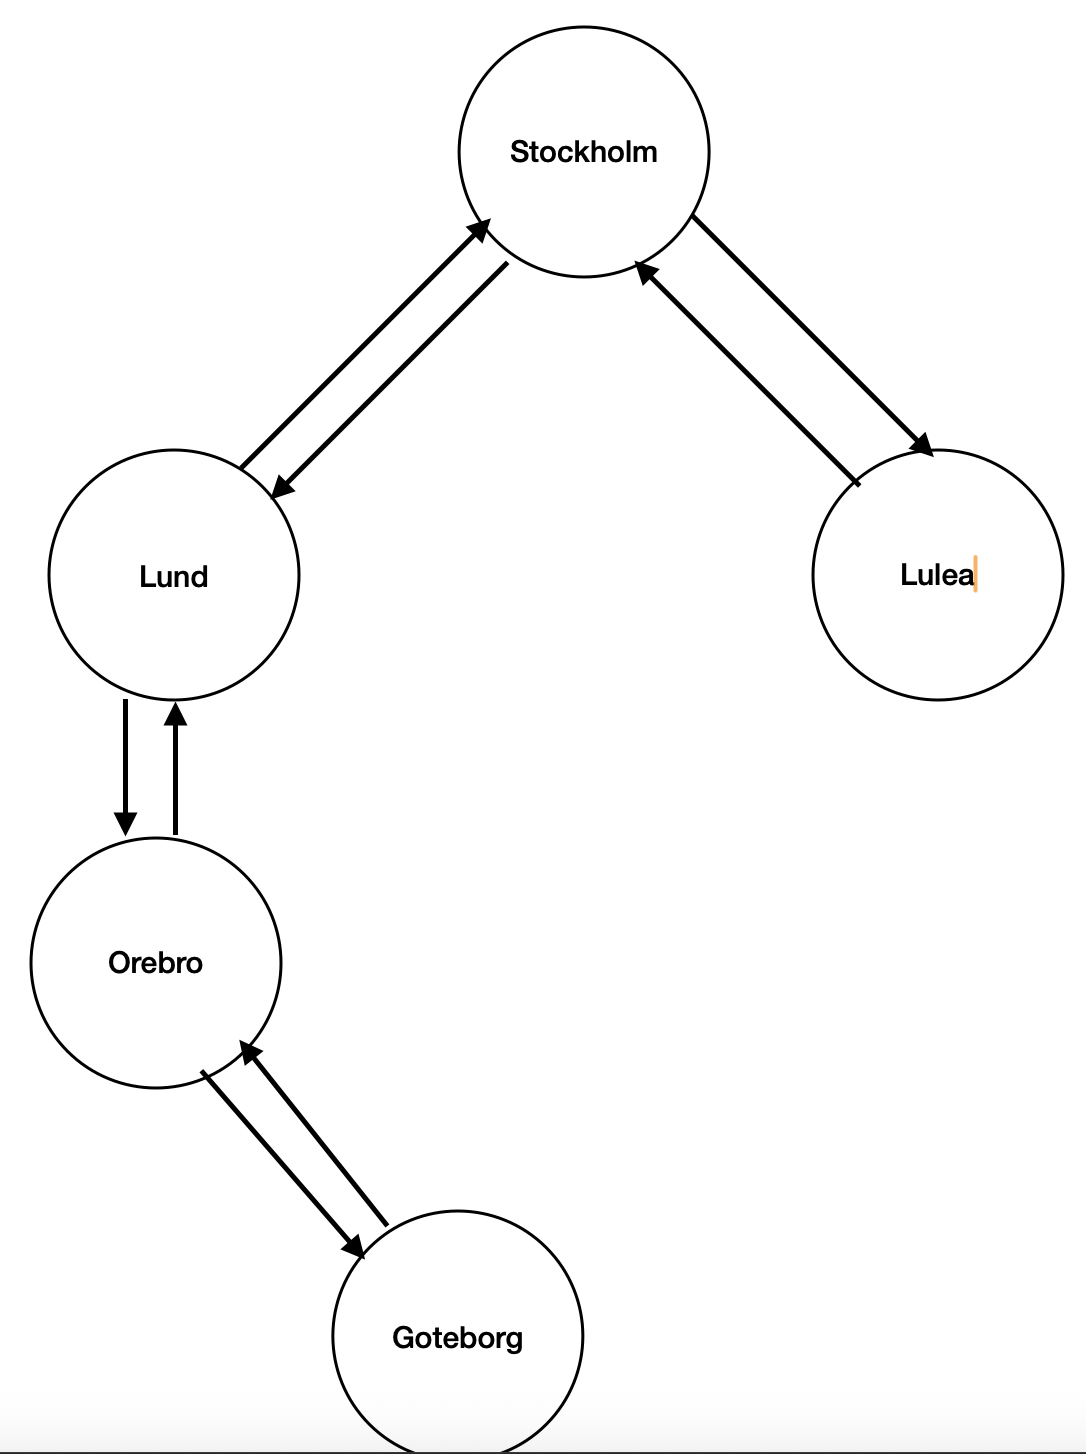
\includegraphics[width=0.4\textwidth]{screenshots/riccardos_topology.png}
\end{center}

From my topology I will remove the connection between \textbf{Turin} and \textbf{Madrid}. Then we will connect both \textbf{Turin} and \textbf{Madrid} to \textbf{Lulea} the new router that is running in Sweden (Riccardo's network).

Let's set up the network and see if the routing still works. This is the result of calling msg:status({r3, 'italy@DORORO'}, 1000).

\begin{center}
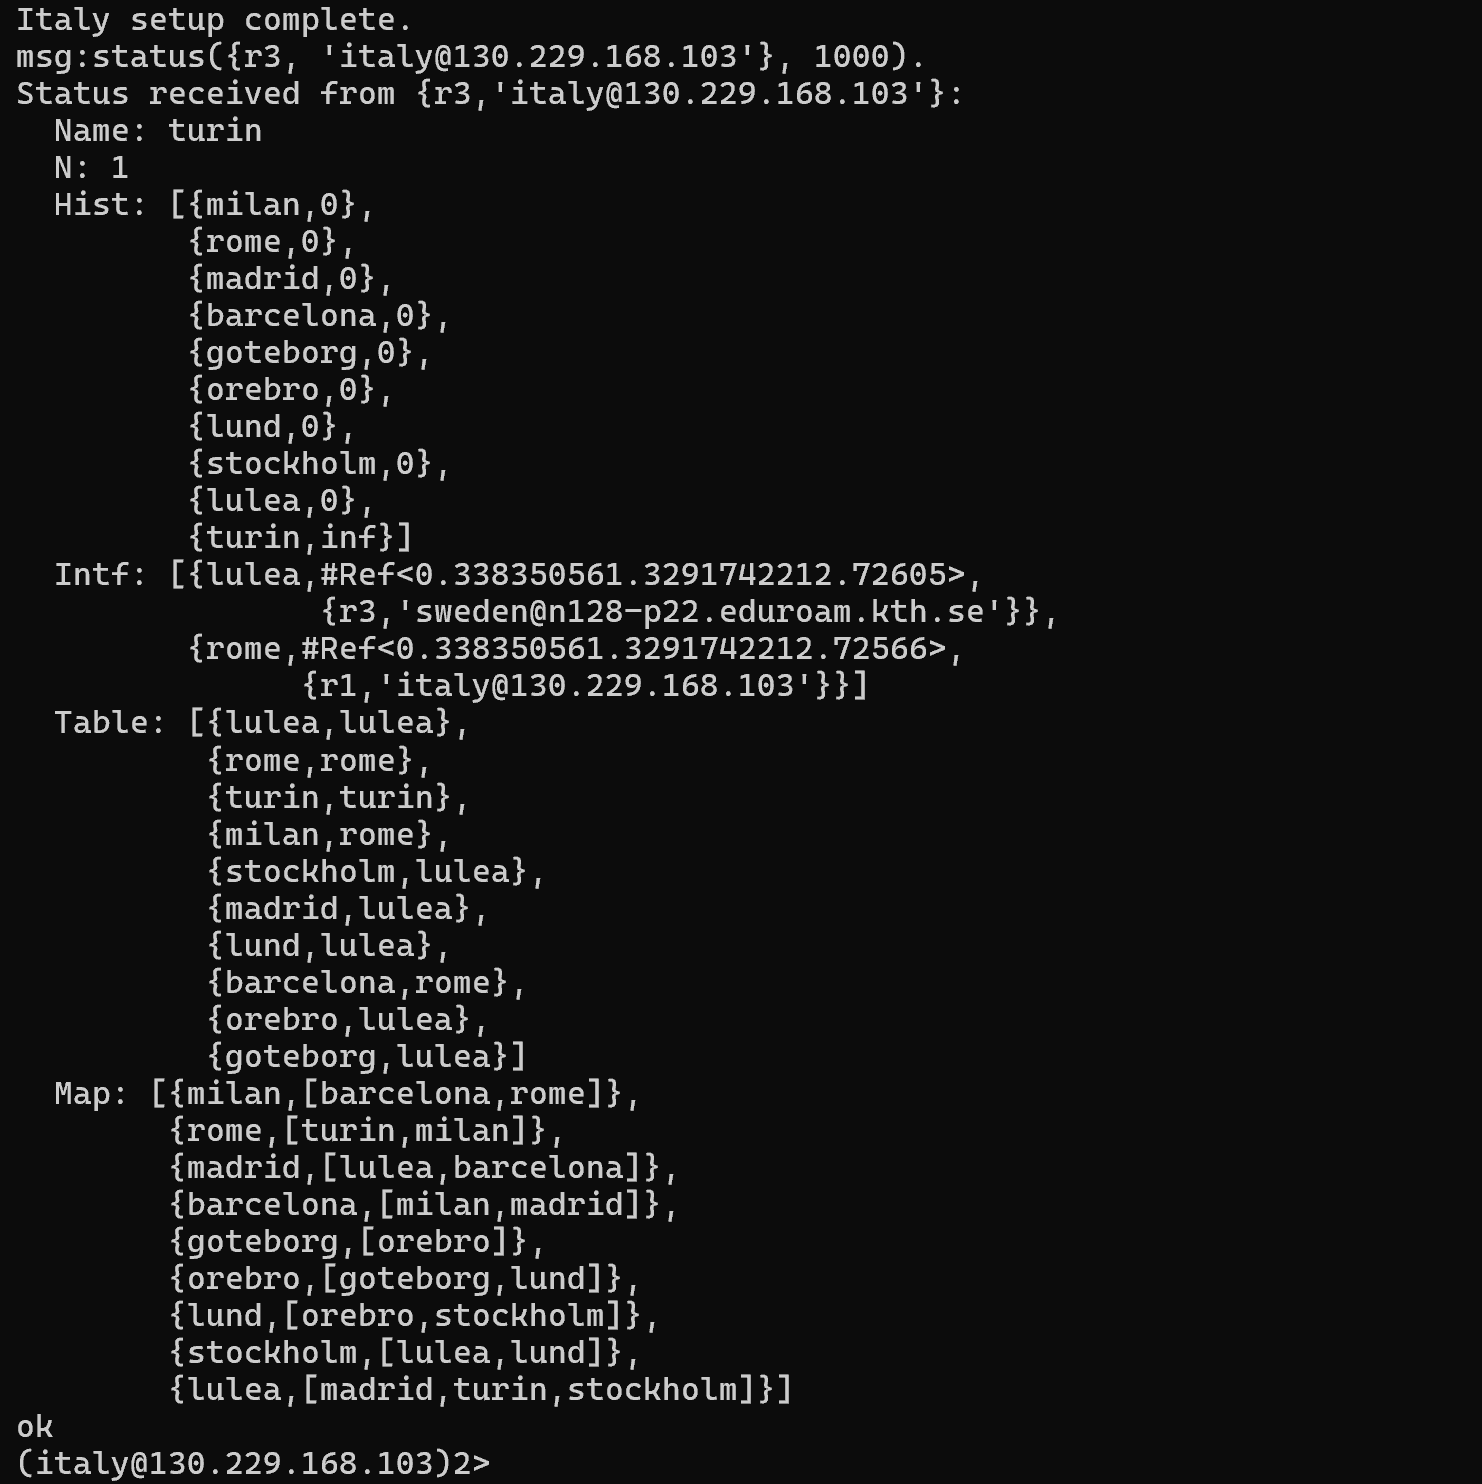
\includegraphics[width=0.8\textwidth]{screenshots/initial_status.png}
\end{center}

Perfect, we can see that the routing tables are correclty set up. Now let's try to send a message from Turin to Madrid. This, time there is a new shortest path that goes through Lulea.

\begin{center}
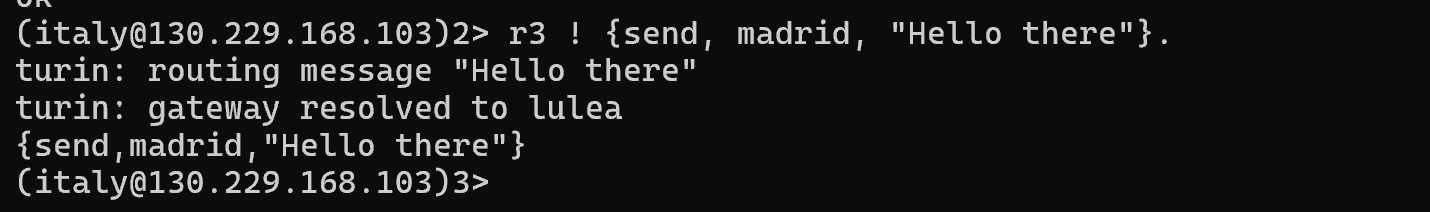
\includegraphics[width=0.8\textwidth]{screenshots/initial_message_routing_to_lulea.png}
\end{center}

Turin sends a message to lulea, which then forwards it to Madrid. The message is correctly routed through the new path: \textbf{Turin} $\to$ \textbf{Lulea} $\to$ \textbf{Madrid}.

\begin{center}
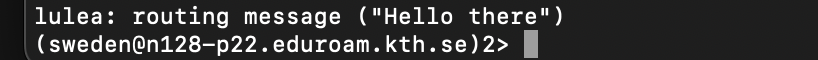
\includegraphics[width=0.8\textwidth]{screenshots/Message_Routing_to_Madrid_From_Lullea.png}
\end{center}

\begin{center}
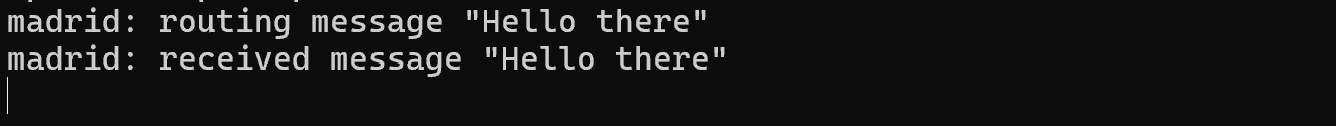
\includegraphics[width=0.8\textwidth]{screenshots/madrid_receives_from_lulea.png}
\end{center}

Let's now see what happens if we kill the erlang process running on Riccardo's machine. This simulates a complete failure of the Sweden area.

\begin{center}
\includegraphics[width=0.8\textwidth]{screenshots/Initial_kill.png}
\end{center}

After sending a kill message to Sweden, on my machine I get:

\begin{verbatim}
turin: exit received from lulea at timestamp 1758108122792
madrid: exit received from lulea at timestamp 1758108122791
\end{verbatim}

Looking at the timestamp from Riccardo's machine (1758108121) we can see that after 1 second both Turin and Madrid have detected the failure of Lulea.

Now, let's try to send a message from Turin to Madrid again:
\begin{center}
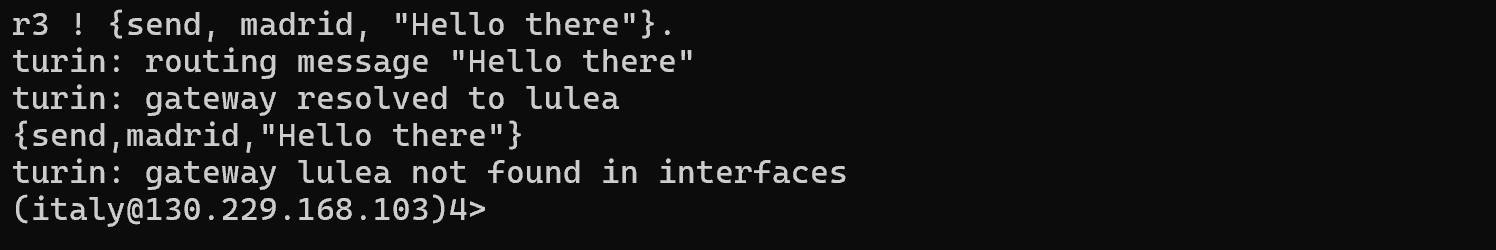
\includegraphics[width=0.8\textwidth]{screenshots/routing_failed.png}
\end{center}

The message routing fails, as expected, because there is no available path between Turin and Madrid after the failure of Lulea.

To wrap it up let's update the routing tables in both areas and send a message again from Turin.
\begin{center}
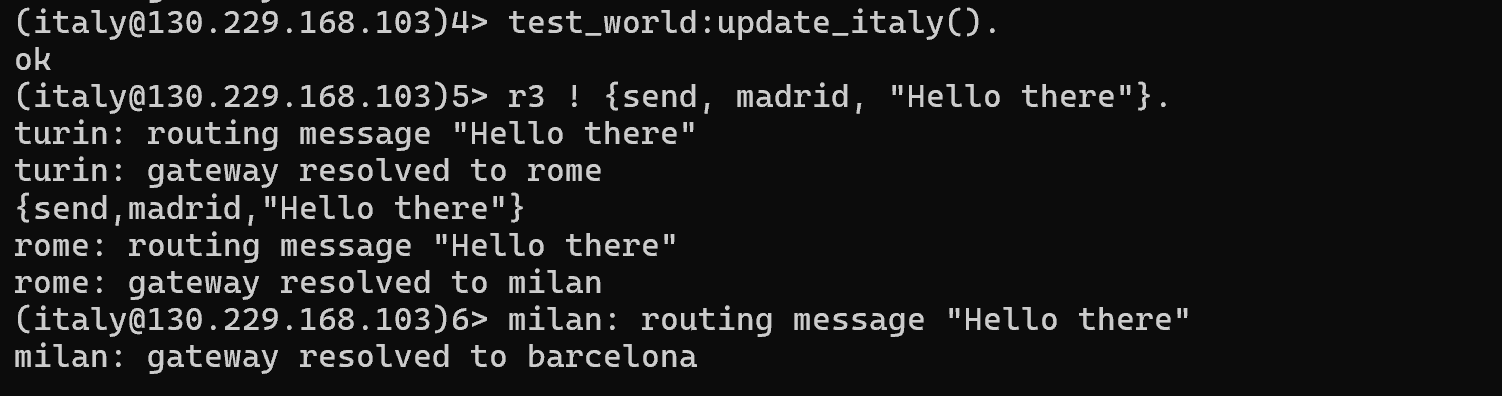
\includegraphics[width=0.8\textwidth]{screenshots/routing_resolved_to_barcelona.png}
\end{center}

\begin{center}
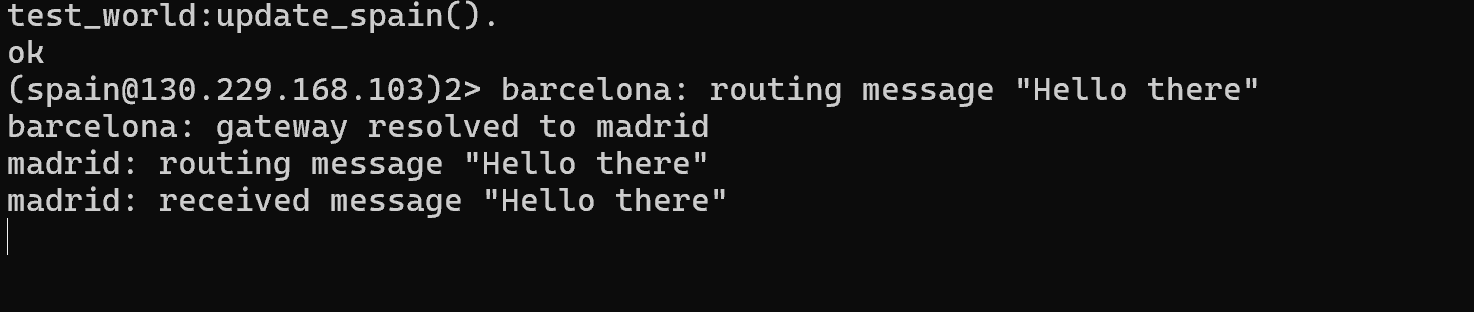
\includegraphics[width=0.8\textwidth]{screenshots/madrid_receives_from_turin.png}
\end{center}

As we can see, the message is correctly routed through the new path: \textbf{Turin} $\to$\ \textbf{Rome} $\to$ \textbf{Milan} $\to$ \textbf{Barcelona} $\to$ \textbf{Madrid}.

\end{document}